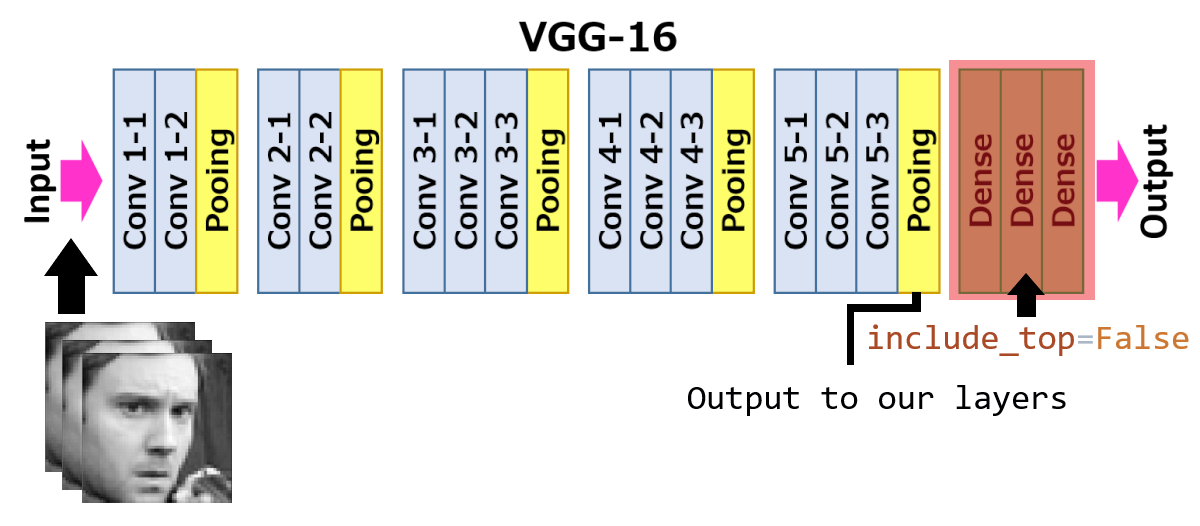
\includegraphics[scale=0.5]{images/modelOne/vgg16layers.png}
At the beginning VGG16 model must be implemented to our environment, in Keras it very easy:
\begin{lstlisting}[language=Python]
    vgg16 = VGG16(include_top=False,
                input_shape=(48, 48, 3),
                pooling='avg',
                weights='imagenet')
\end{lstlisting}

There are two ways to use pretrained model:
\begin{itemize}
          \item train whole model with vgg16 frozen layers
          \item get vgg16 output and train our model (final layers) separately
\end{itemize}
First idea took too much time to train.
More efficient way is to get output of VGG16 and then proceed through our layers and train only a few layers.\\
After that two models are combinded: VGG16 + our layers.\\
This is a presentation of model in Keras: last two layers of frozen VGG16 and out final model\\
\begin{center}
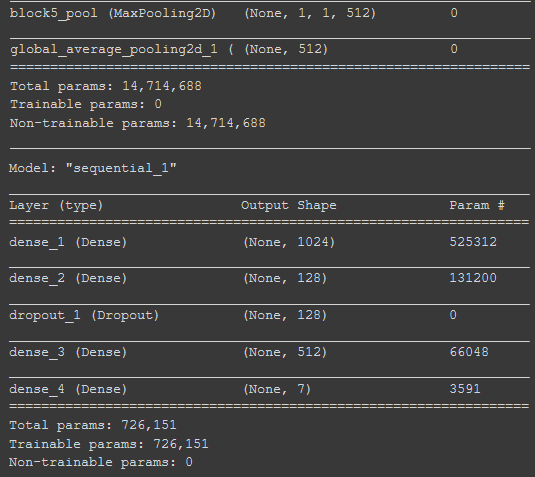
\includegraphics[scale=0.75]{images/modelOne/modelKeras.png}
\end{center}

